\chapter{User's Manual} \label{sec:manual}

This manual will describe the impedance spectrometer in detail and give step by step instructions for using it.

An overview of the device connections can be seen in \autoref{fig:device_connections}, when referring to connectors
later, the numbers from the image will be used in bold font. Connector footprints for unimplemented features are not
labeled, the push buttons on the board are the same as those on the STM32F4 Discovery board.

\begin{figure}[htpb]
  \centering
    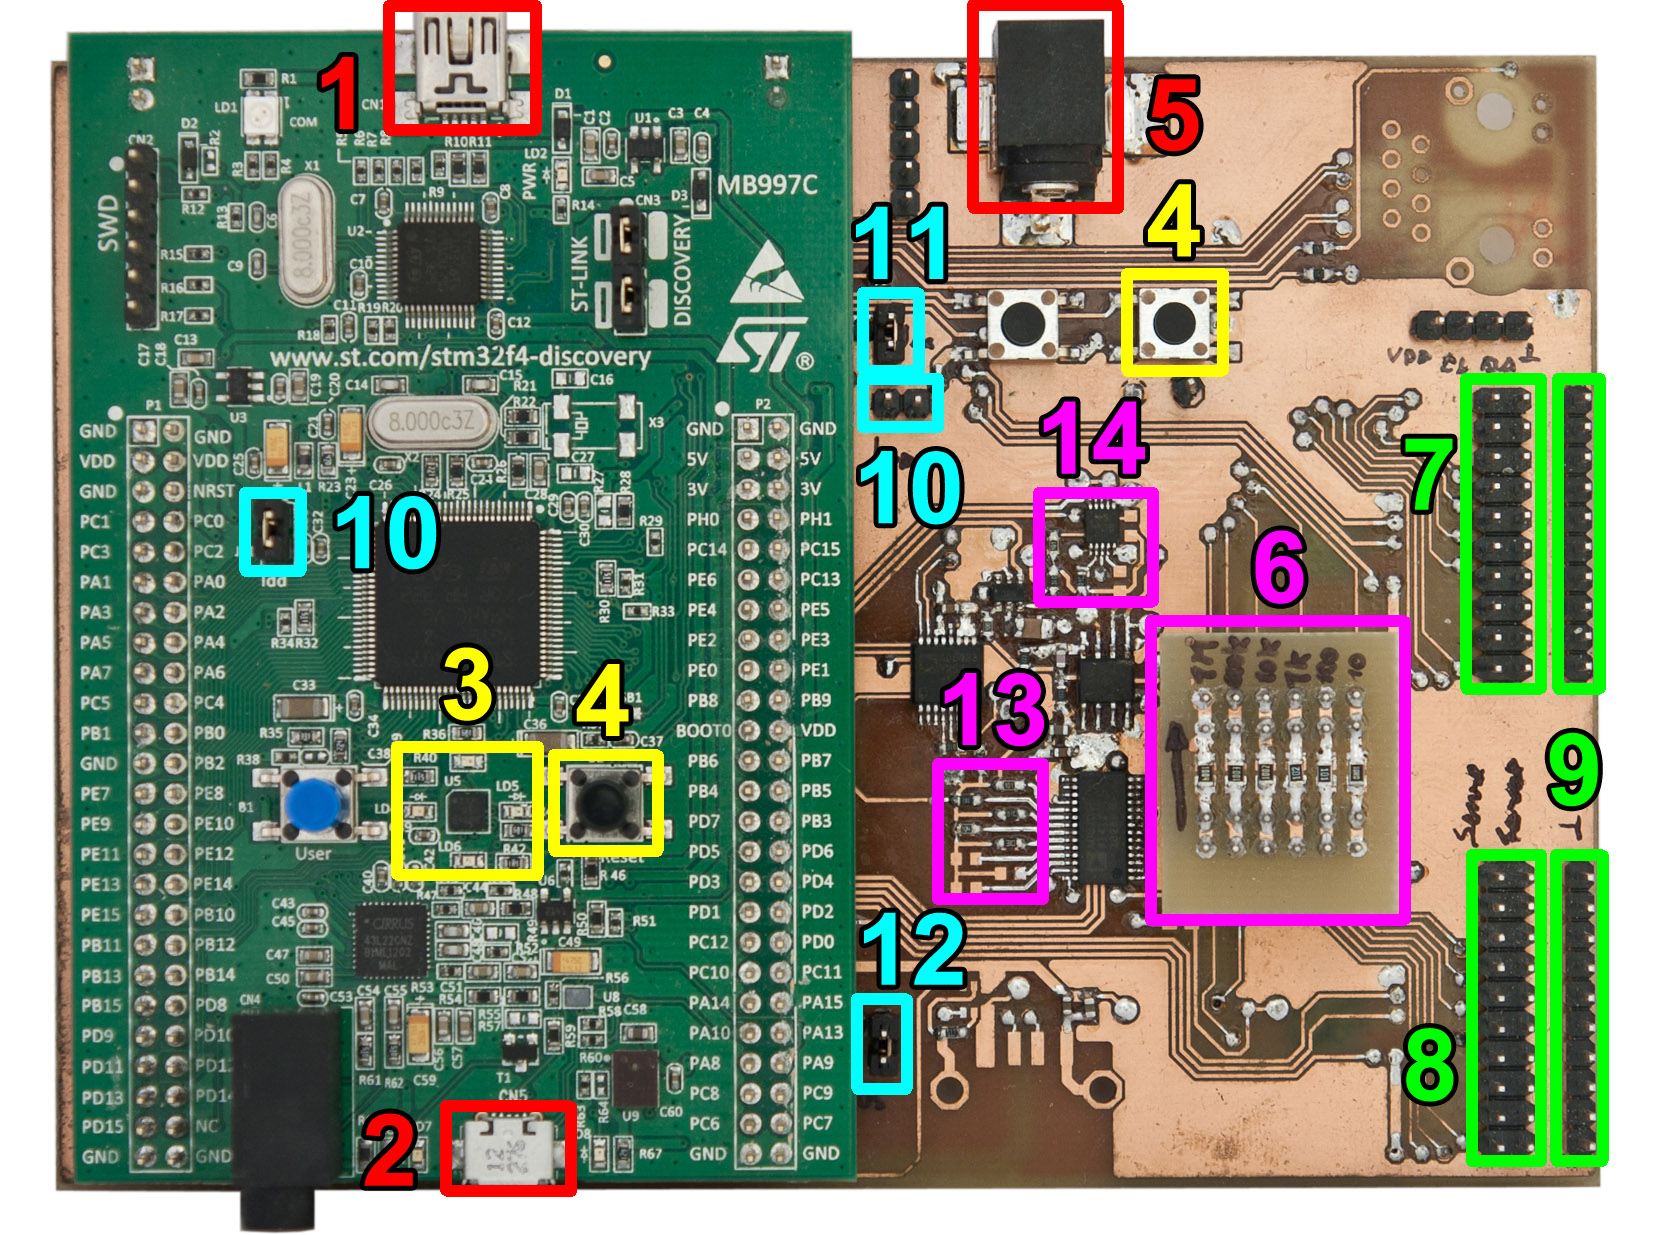
\includegraphics[width=\textwidth]{bilder/device_connections.jpg}
  \caption[Interface on the assembled impedance spectrometer]{
    Interface on the assembled impedance spectrometer:
    \begin{enumerate*}[label=\textbf{\arabic*}, itemjoin={{ -- }}]
      \item USB programming and power connector
      \item device USB connector
      \item status LEDs
      \item reset button
      \item DC power jack
      \item board with calibration resistors
      \item measurement output connections, sense (left) and force (right)
      \item measurement input connections (same as output)
      \item ground connections
      \item $ I_\text{DD} $ measurement jumper
      \item $ I_\text{CC} $ measurement jumper
      \item $ V_\text{BUS} $ jumper
    \end{enumerate*} }
  \label{fig:device_connections}
\end{figure}

